%%%%%%%%%%%%%%%%%%%%%%%%%%%%%%%%%%%%%%%%%%%%%%%%%%%%%%
\chapter{Experimental design}
\label{experimental_design}
\graphicspath{{chapter_03/figures}{chapter_03/tables}}
%%%%%%%%%%%%%%%%%%%%%%%%%%%%%%%%%%%%%%%%%%%%%%%%%%%%%%





\section{Development of the multi-parameter data-driven forecasts of areas at risk of flash flood}

Traditional physically-based models, which rely on physical equations and mathematical models, are the backbone of many scientific disciplines for decades. These algorithms are based on well-established principles and laws of physics, enabling a systematic and predictable approach to problem-solving. On the other hand, AI-based strategies emerge as a powerful tool for handling vast amounts of data and extracting patterns and relationships that might be challenging to identify through traditional algorithms.

Over the years, semi-empirical, index-based models have provided predictions of areas at risk of flash floods up to continental scales \citep{Ma_2021} and medium-range lead times \citep{Alfieri_2015a, Raynaud_2015}. However, their extension to a global domain remains difficult because to set all free parameters over a region of interest or global domain, a large amount of flash flood observations (either form discharge gauges or impact reports) are needed and, to this day, this is a requirement still difficult to satisfy being flash floods rare events, happening typically in ungauged catchments, and being largely underreported in impact databases. 

Alternative strategies to deal with the issue of forecasting exploit data-driven-based predictions, defined as predictions made solely in terms of the knowledge of field data. Recently, data-driven methods have shown potential in accelerating weather forecasting by orders of magnitude, even if the accuracy of the forecasts is not always higher than that of NWP models \citep{Bauer_2021}. To date, there are a series of data-driven models that learn meteorological \citep{Lang_2024} and hydrological \citep{Nearing_2024} dynamics from ERA5 global reanalysis. However, ERA5 does present limitations in reconstructing sub-grid features due to the coarse spatial resolution, inherent biases in the model, and sub-grid processes that are only parametrised in the NWP model \citep{Pillosu_2025a}. Hence, the same skills shown in previous literature should not be taken for granted when the focus is on the representation of phenomena that occur at sub-grid scale or for extreme events (e.g. rainfall events exceeding, for example, the 20-year return period or larger thresholds).

Data-driven approaches have been used widely to forecast flash flood events, but primarily up to 24-hours ahead and solely at catchment \citep{Zhao_2025, Saleh_2024, Oddo_2024}, regional \citep{Deijns_2024}, and national level \citep{Villacca_2025, Zhao_2022}. While achieving very good verification scores (for example AROC scores > 0.8), the use of such data-intensive, data-driven algorithms, such as deep neural networks is not possible for global applications. While recent wisdom advocates for using hydro-meteorological data for a number of catchments available around the world to train a single model that later can be used to provide seamless flood forecasts around the world \citep{Kratzert_2024}, the application of similar strategies is restricted for flash flood applications due to the rather small number of data available for flashy catchments around the world e.g., 1\% of catchments in the CARAVAN database have an area below <100 km2 \citep{Kratzert_2023}. Even including more recent extensions of the CARAVAN database, such the percentage of data for flashy catchments does not exceed 5\% of the full database \citep{Färber_2024}.

Less data-intensive machine learning algorithms, such as decision-tree-based algorithms, such as random forest and boosting, and shallow feed-forward neural networks, could help to model the non-linear relationships between the hydro-meteorological parameters and create predictions of areas at risk of flash floods even when using low-density impact flash flood impact databases. The aim is to train the data-driven model with the higher-resolution Storm Event Database and apply it globally to provide predictions over a continuous global domain, for short-range forecasts (up to day 1) using ERA5 short-range forecasts (aka reanalysis) and for medium-range forecasts (up to day 5) using ERA5 long-range forecasts.

\subsection{The challenge of imbalanced observational datasets}

\subsubsection{Ensemble techniques}
The resulting observational dataset, built as described in section \ref{obs_field} is strongly imbalanced, with only 0.2\% of yes-events over the whole training+testing period (from 2001 to 2024). Using a similar dataset for the learning stage of our data-driven model is challenging, as the model might learn that non-events should always be predicted, as the model sees too few yes-events compared to the non-events, so that the model gives up on predicting the yes-events \citep{Haixiang_2017}. To overcome this problem, different techniques at data-level or algorithm-level are available \citep{Altalhan_2025}. 

Data-level balancing techniques focus on aligning class distributions by adjusting the size of training datasets through resampling, which aims to equalise the class distribution through "undersampling" or "oversampling" approaches. Standard undersampling techniques include Random Undersampling, Tomek, and cluster centroids, while prominent oversampling techniques include SMOTE and derivatives like Borderline-SMOTE and ADASYN \citep{DeVargas_2023}. However, these approaches introduce two main challenges: oversampling may lead to overfitting, reducing generalisation on the test set, whereas undersampling may result in a significant loss of knowledge from the majority class (i.e. non-events). Generative Adversarial Networks (GANs) are also used to improve the classification accuracy of imbalanced datasets. Oversampling and GAN techniques generate synthetic samples and the verification of how their distribution if to that of the original dataset is very difficult due to the lack of real observational data. Hence, we might be training models with data that does not respect the frequency distribution of yes-(flash flood)events.

Algorithm-level techniques enhance learning in the minority class by immediately altering the training process of the classifier or modifying algorithms to address challenges associated with imbalanced datasets \citep{Altalhan_2025}. Algorithm-specific adjustments like adapting class-balanced loss functions for gradient Boosting Decision Trees have shown high effectiveness in addressing class imbalance \citep{Luo_2025}. Ensemble methods entail merging multiple base classifiers or models to forge a more robust learner to address the imbalance problem, such as random forest, gradient boosting, bagging, and stacked learning. These approaches leveraged various algorithms or versions of the same model (e.g. for extreme gradient boosting, different version of the same algorithm can be, for example, XGBoost and LightGBM) to bloster predictive performance on imbalance datasets. 

In this thesis we do not apply data-level balancing techniques because we do not want to introduce uncertainties in the estimation of the forecasts by pre-processing the training dataset, either creating synthetic data over oversampling, or eliminating possibly information-riched non-event data-points. To not introduce uncertainty in the predictions, we will not consider algorithm-specific adjustments either. To consider these techniques robustly, a thorough assessment of each technique would be needed, using predictions from models trained on the original "real" observations as a benchmark to assess any gain or loss of predictive performance in the models trained with modified training datasets or modified algorithms. This work is out of the scope of this thesis. For future work in this field, the results produced in this thesis might serve as benchmark for those predictions. Hence, in this study, we will consider ensemble techniques to address the problem of having an extremely imbalnce dataset, and the models mentioned in Table \ref{} will be used. 


\subsubsection{Stratified k-fold cross validation}

Instead of assessing the robustness of the learning process by dividing the observational dataset into training, validation, and test sets, training only once over the training dataset and evaluating the model only once over the validation and test dataset, we opted for a validation strategy that allows for controlling the robustness of the inference phase. A well-established approach for this scope is the " stratified k-fold cross-validation", where possible biases caused by a fortunate/ unfortunate choice of the test dataset are mitigated by selecting different training, validation, and test datasets at each iteration. 

The core of the methodology lies in a nested cross-validation with hyperparameter tuning (see workflow in Figure \ref{fig:train_model}). 

\begin{figure}[htbp]
\centering
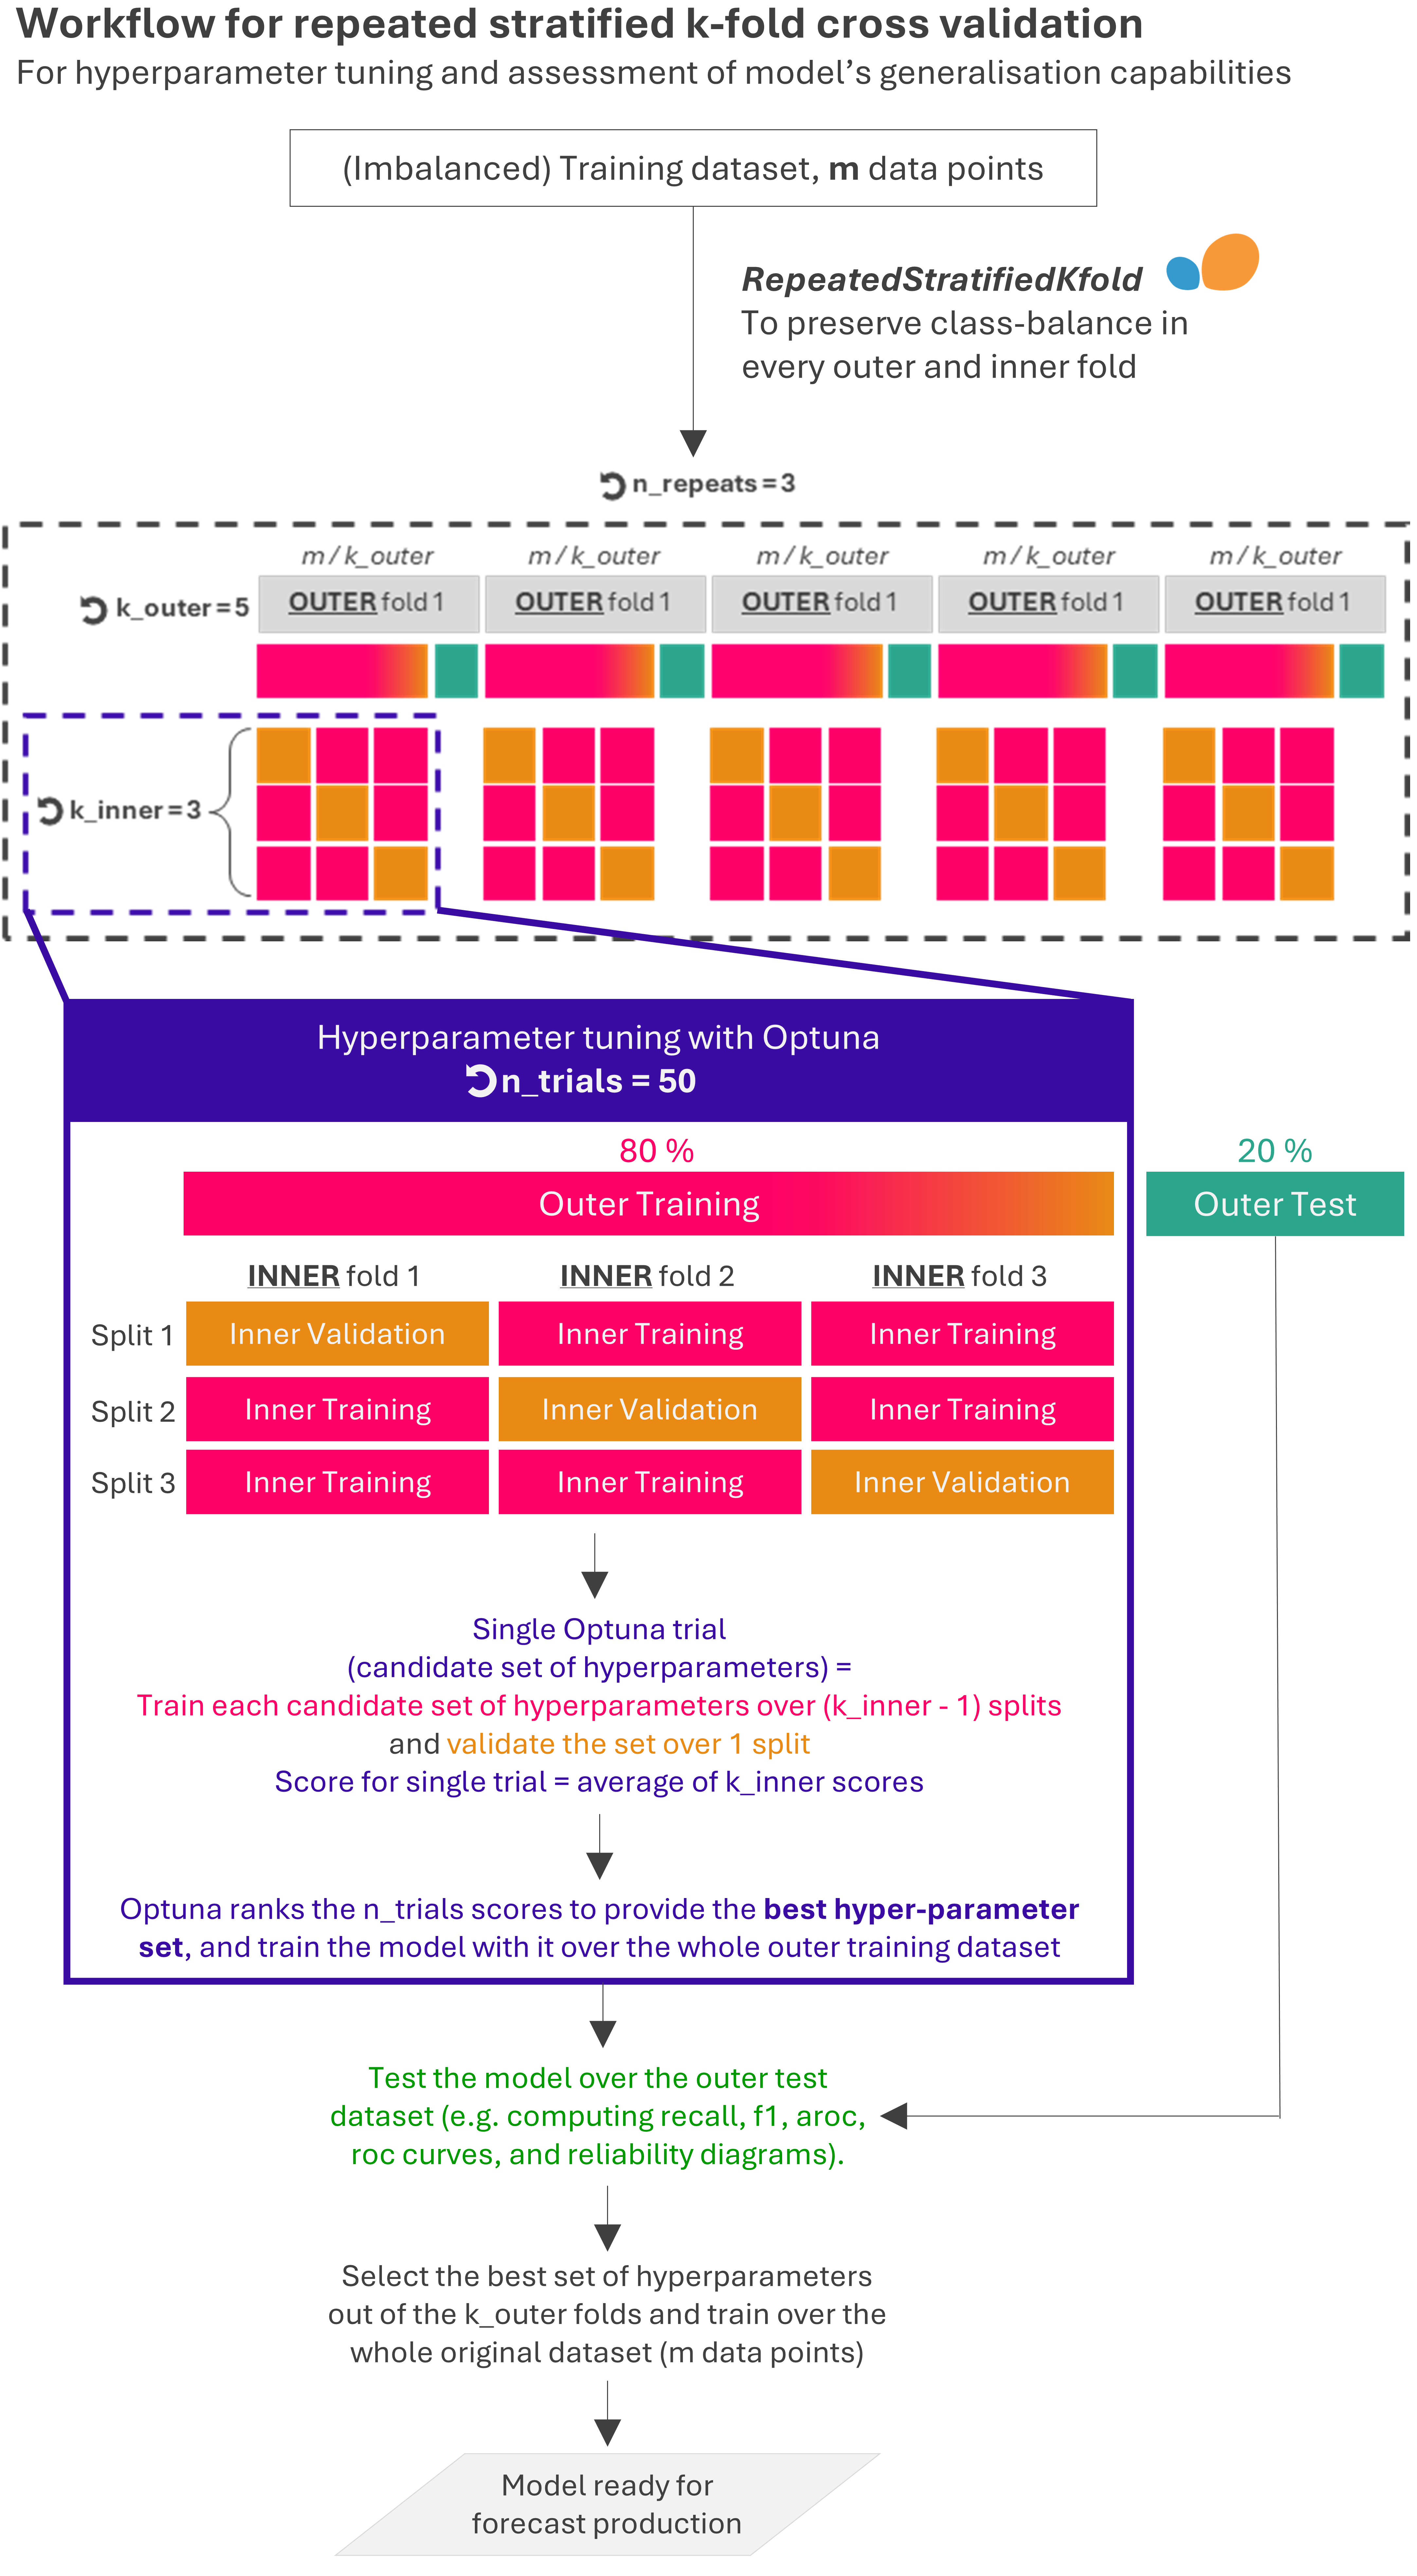
\includegraphics[width=\textwidth]{train_model.png}
\caption{\textbf{Repeated Stratified k-fold cross-validation.} Workflow for the Repeated Stratified k-fold cross-validation.}
\label{fig:train_model}
\end{figure}

A nested cross-validation is a technique used to evaluate fine-tune the hyperparameters of a data-driven model while mitigating the risk of overfitting and obtaining biased performance estimates. The technique consists of two nested loops: an outer loop for model evaluation and an inner loop for model hyperparameter tuning. In the outer loop, the data is split into an outer training and test datasets using the repeated stratified k-fold cross-validation. This loop aims to provide an unbiased estimate of the model's performance on unseen data (i.e. the outer test data). The outer loop was implemented using Scikit-learn's function \textit{RepeatedStratifiedKFold} with n\_outer splits and n\_repeats repetitions. The stratification ensures that the class distribution in each fold is representative of the entire dataset, which is particularly important for imbalanced datasets like the one used in this thesis. n\_outer = 5 splits and n\_repeats = 1 repetitions will be considered. n\_repeats = 5 will be considered if the results look unstable. 

Within each iteration of the outer loop, the inner loop is executed. The inner loop focuses on hyperparameter tuning. It takes the outer training data and further splits it into inner training and inner validation sets. The purpose of the inner loop is to find the best combination of hyperparameters for the considered model (e.g. random forest, boosting, etc.) using a specified search strategy, such as grid search, random search. In this thesis, Optuna was used. Also over the inner loops, it is applied a repeated stratified k-fold cross-validation, with n\_inner = 3 loops and n\_trials = 20 repetitions. Over each inner fold, the model's performance is evaluated. In this thesis, the AROC metric was used. The mean of the AROC scores over all inner folds is returned to be maximised by Optuna. After the inner loops finish, the best-performing models and its hyperparameters are selected. After the hyperparameter optimisation process, the best hyperparameters found by Optuna are used to train a final model on the entire outer train split. This model is then evaluated on the outer loop's test dataset, which was held out and not used during the hyperparameter tuning, providing an unbiased estimated of the model's performance on unseen data. Various performance metrics such as F1 score, recall, AROC, frequency bias and reliability diagrams are computed. 

The process repeats for each iteration of the outer\_loop, resulting in n\_outer performance estimates, one for each outer fold. The final performance of the model is typically reported as the average and standard deviation of these estimates, providing a more robust and reliable assessment of the model's generalisation ability.

The nested cross-validation approach has several advantages: (1) it provides an unbiased estimate of the model's performance, as the test data in the outer loop is never used for hyperparameter tuning, (2) it allows for the selection of the best model and hyperparameters based on the inner loop's validation performance, reducing the risk of overfitting, and (3) by repeating the outer loop n\_outer times, it captures the variability in the model's performance, providing a more comprehensive understanding of its behaviour. However, nested cross-validation can be computationally expensive, especially when dealing with large datasets or complex models.

Optuna's hyperparameter search was used due to its efficiency as it employs an optimisation algorithm called "Tree-structured Parzen Estimator", which intelligently suggests hyperparameter combinations based on past trials. This allows Optuna to find a well-performing hyperparameter configuration more quickly, reducing the overall computational cost. Optuna is also extremely flexible, supporting various data types (e.g., integers, floats, and categorical) and specifying distributions (e.g. uniform, log-uniform) from which the hyperparameter values are sampled. This flexibility enables exploring a wider range of hyperparameter combinations compared to other methods. Optuna also has built-in support for parallelisation, allowing multiple trials to be executed concurrently. This feature can significantly speed up the hyperparameter tuning process, especially when dealing with large datasets and complex models. Optuna also incorporates a pruning mechanism that allows for the early stopping of unpromising trials. Hence, by leveraging Optuna's advanced hyperparameter tuning capabilities, the code can explore a broader range of hyperparameter configurations, find well-performing models more quickly, and potentially achieve better predictive performance than using grid or random search alone.

\subsubsection{Data-driven models}
The following models were used in this thesis:

\begin{itemize}
    
    \item \textbf{Random Forest:} random forest model, is an ensemble learning method where each tree is trained on a randomly selected subset of the training data and features, introducing diversity and reducing overfitting. The final prediction is obtained by aggregating the outputs of the individual trees. XGBoost's implementation of Random Forest offers advantages such as parallel processing, regularisation techniques, and efficient handling of missing values. It is known for its robustness, scalability, and ability to handle complex nonlinear relationships in the data. LightGBM's implementation is designed to be highly efficient and scalable, making it suitable for large datasets. It employs techniques such as gradient-based one-side sampling (GOSS) and exclusive feature bundling (EFB) to accelerate training and reduce memory usage. LightGBM's Random Forest model is known for its fast training speed, low memory requirements, and ability to handle categorical features directly, without the need for one-hot encoding.
    
    \item \textbf{Adaptive Boosting:} adaptive boosting, is an ensemble learning method that combines multiple weak learners (usually decision trees) to create a strong classifier. It iteratively trains the weak learners, assigning higher weights to misclassified instances in each iteration. This focusing on difficult examples helps the model to improve its performance. AdaBoost is known for its simplicity, theoretical foundations, and ability to handle noisy data. However, it can be sensitive to outliers and may overfit if the weak learners are too complex. AdaBoost's Gradient Boosting implementation provides a straightforward and effective approach to ensemble learning.
    
    \item \textbf{Gradient Boosting:} gradient boosting is an ensemble learning method that combines weak learners (typically decision trees) in an iterative fashion. Each tree is trained to correct the errors made by the previous trees, allowing the model to gradually improve its predictions. XGBoost's Gradient Boosting implementation includes several advanced features, such as regularisation techniques (L1 and L2), tree pruning, and built-in cross-validation. It is known for its strong predictive performance, ability to handle complex relationships, and robustness to outliers and missing data. LightGBM's implementation focuses on efficiency and scalability, using techniques like GOSS and EFB to speed up training and reduce memory consumption. It also supports leaf-wise tree growth, which can lead to more accurate models compared to level-wise growth used in other implementations. LightGBM's Gradient Boosting model is known for its fast training speed, low memory usage, and ability to handle large datasets effectively. CatBoost's implementation uses a technique called ordered boosting, which permutes the training data to reduce overfitting on categorical variables. CatBoost also employs symmetric trees, which ensure that the model is invariant to the order of categories in categorical features. Additionally, it includes advanced features like automatic handling of categorical variables, feature combinations, and built-in overfitting detection. CatBoost's Gradient Boosting model is known for its strong performance on datasets with complex categorical features and its ability to produce highly accurate predictions.
    
    \item \textbf{Feed-forward shallow neural network:} the shallow feed-forward neural network, implemented using the Keras library, is a type of artificial neural network where the information flows in one direction, from the input layer to the output layer, through one or more hidden layers. Each layer consists of interconnected nodes (neurons) that apply nonlinear transformations to the input data. The network learns to map the input features to the target variable by adjusting the weights of the connections during training, using optimisation algorithms like stochastic gradient descent. Feed-Forward Neural Networks are capable of learning complex nonlinear relationships and can be effective for a wide range of prediction tasks, including flash flood prediction.

\end{itemize}

While those models, with the exception of the feed-forward neural network, are all considered ensemble models, they are built with using multiple but the same model types, e.g. random forest uses only decision trees. To complement these models, ensemble techniques that blend the predictions from different model types are also considered:


\begin{itemize}
    
    \item \textbf{Bagging:} Bagging, short for Bootstrap Aggregating, is an ensemble technique that combines multiple base models trained on different subsets of the training data. It involves creating bootstrap samples (random samples with replacement) from the original training data and training a separate model on each sample. The predictions of the base models are then aggregated, typically through averaging or voting, to obtain the final prediction. Bagging helps to reduce overfitting and improve the stability and robustness of the ensemble model. It is particularly effective when the base models are unstable or prone to overfitting, such as decision trees. Bagging can be applied to various types of base models, including the random forest and gradient boosting models considered in this study.
    
    \item \textbf{Stacking:} Stacking, also known as stacked generalization, is an ensemble technique that combines the predictions of multiple base models by training a meta-model on top of their outputs. The base models are first trained on the original training data, and their predictions on a validation set are used as input features for the meta-model. The meta-model learns how to optimally combine the predictions of the base models to make the final prediction. Stacking allows for the integration of diverse base models, potentially capturing different aspects of the data and improving the overall predictive performance. The meta-model can be any algorithm capable of learning from the base model predictions, such as logistic regression, random forest, or gradient boosting. Stacking is a powerful ensemble technique that can leverage the strengths of individual models and provide a higher level of abstraction in the learning process.

\end{itemize}


\subsubsection{Verification scores considered for the data-driven forecasts}
After determining the best set of hyperparameters for each individual model through the nested cross-validation process, the next step is to evaluate the performance of these optimised models using a comprehensive set of metrics. The selected evaluation metrics include:

\begin{itemize}
  \item \textbf{F1 score:} The F1 score is the harmonic mean of precision and recall, providing a balanced measure of the model's ability to correctly identify positive instances while minimizing false positives and false negatives. It is particularly useful when dealing with imbalanced datasets, such as those often encountered in flash flood prediction.
  \item \textbf{Recall:} Recall, also known as sensitivity or true positive rate, measures the proportion of actual positive instances that are correctly identified by the model. In the context of flash flood prediction, high recall indicates that the model is able to correctly identify a large proportion of the actual flood events.
  \item \textbf{Area Under the ROC curve, AROC}: The AROC is a performance metric that evaluates the model's ability to discriminate between positive and negative instances across different classification thresholds. It plots the true positive rate against the false positive rate, providing an aggregate measure of the model's performance. A higher AROC value indicates better overall performance.
  \item \textbf{Frequency bias, FB:} Frequency bias measures the ratio of the number of predicted positive instances to the number of actual positive instances. It assesses whether the model tends to overpredict (frequency bias > 1) or underpredict (frequency bias < 1) the occurrence of flash floods. A frequency bias close to 1 indicates that the model's predictions are well-calibrated with the actual frequency of flash flood events.
  \item \textbf{Reliability diagrams:} Reliability diagrams are graphical representations that compare the predicted probabilities of the model with the observed frequencies of flash flood occurrence. They assess the calibration of the model's predictions, i.e., how well the predicted probabilities align with the actual observed frequencies. A well-calibrated model should have predicted probabilities that closely match the observed frequencies across different probability bins.

\end{itemize}
